% =============================================================================
% Appendix: Supplementary Material
% =============================================================================
% SPDX-FileCopyrightText: 2026 Frank Langbein <frank@langbein.org>
% SPDX-License-Identifier: LPPL-1.3c
%
% Appendices hold supporting material (detailed tables, derivations, survey text,
% user-study materials) so the main narrative stays focused. Complete source
% code is usually submitted separately, not in the report. Use \chapter and
% \section as in main chapters. Replace with your own supplementary material.
% =============================================================================

This appendix contains supplementary material: extra tables, derivations, or notation. Replace with your own content.

\section{Additional data}\label{app:data}

\begin{figure}[htbp]
	\centering
	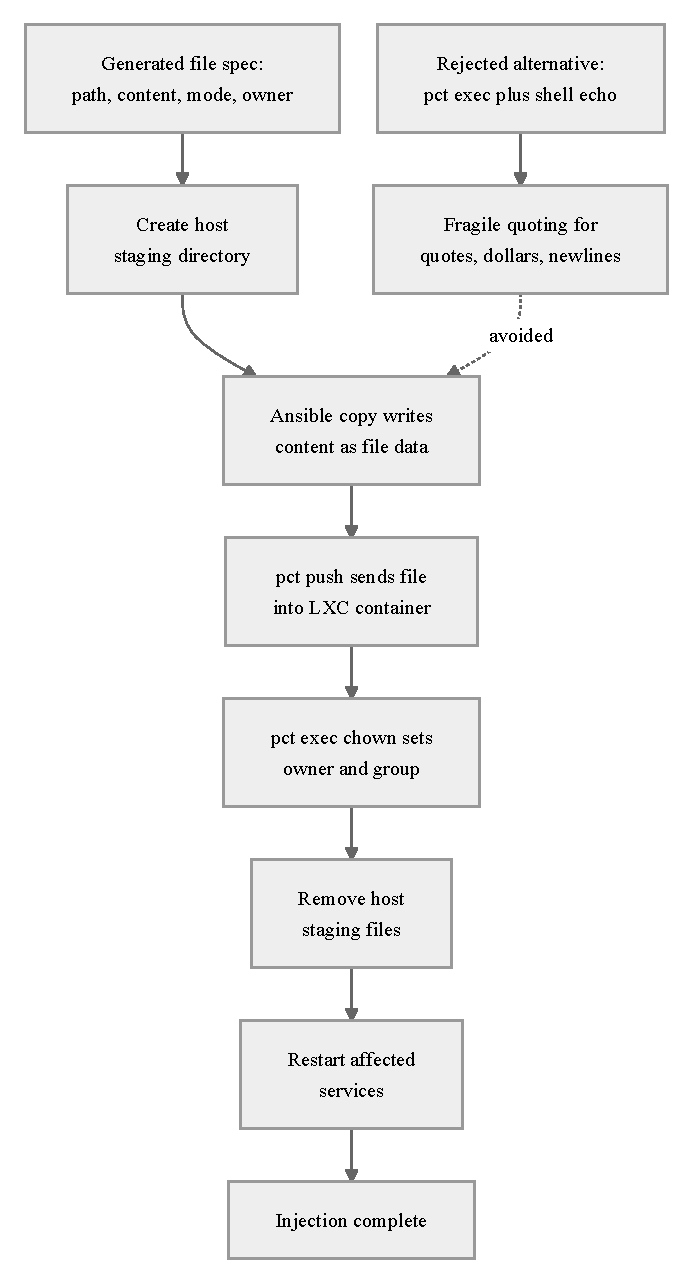
\includegraphics[
		width=\linewidth,
		height=0.82\textheight,
		keepaspectratio
	]{figures/file_injection.pdf}
	\caption{File Injection}
	\label{fig:file_injection}
\end{figure}

\begin{figure}[htbp]
	\centering
	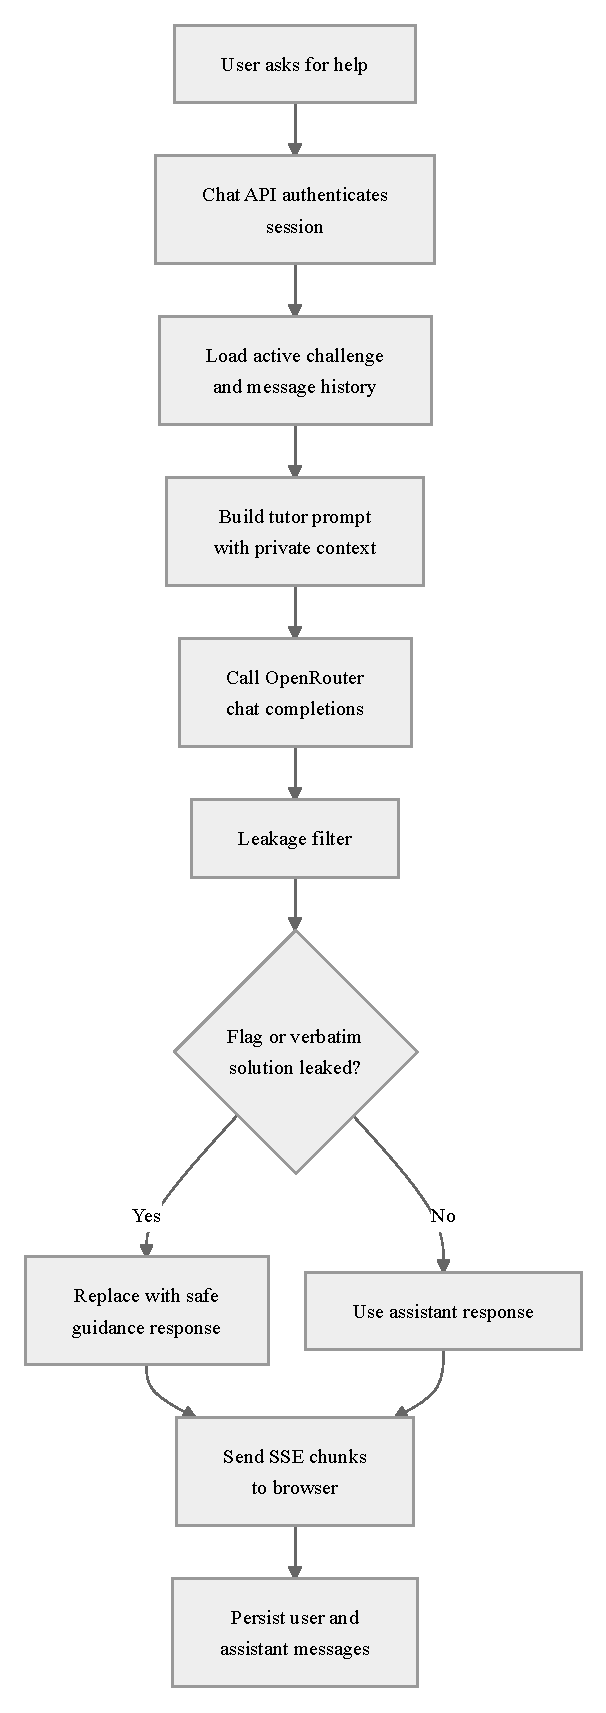
\includegraphics[
		width=\linewidth,
		height=0.82\textheight,
		keepaspectratio
	]{figures/tutor_chat_flow.pdf}
	\caption{Tutor Chat Flow}
	\label{fig:tutor_chat_flow}
\end{figure}

\begin{figure}[htbp]
	\centering
	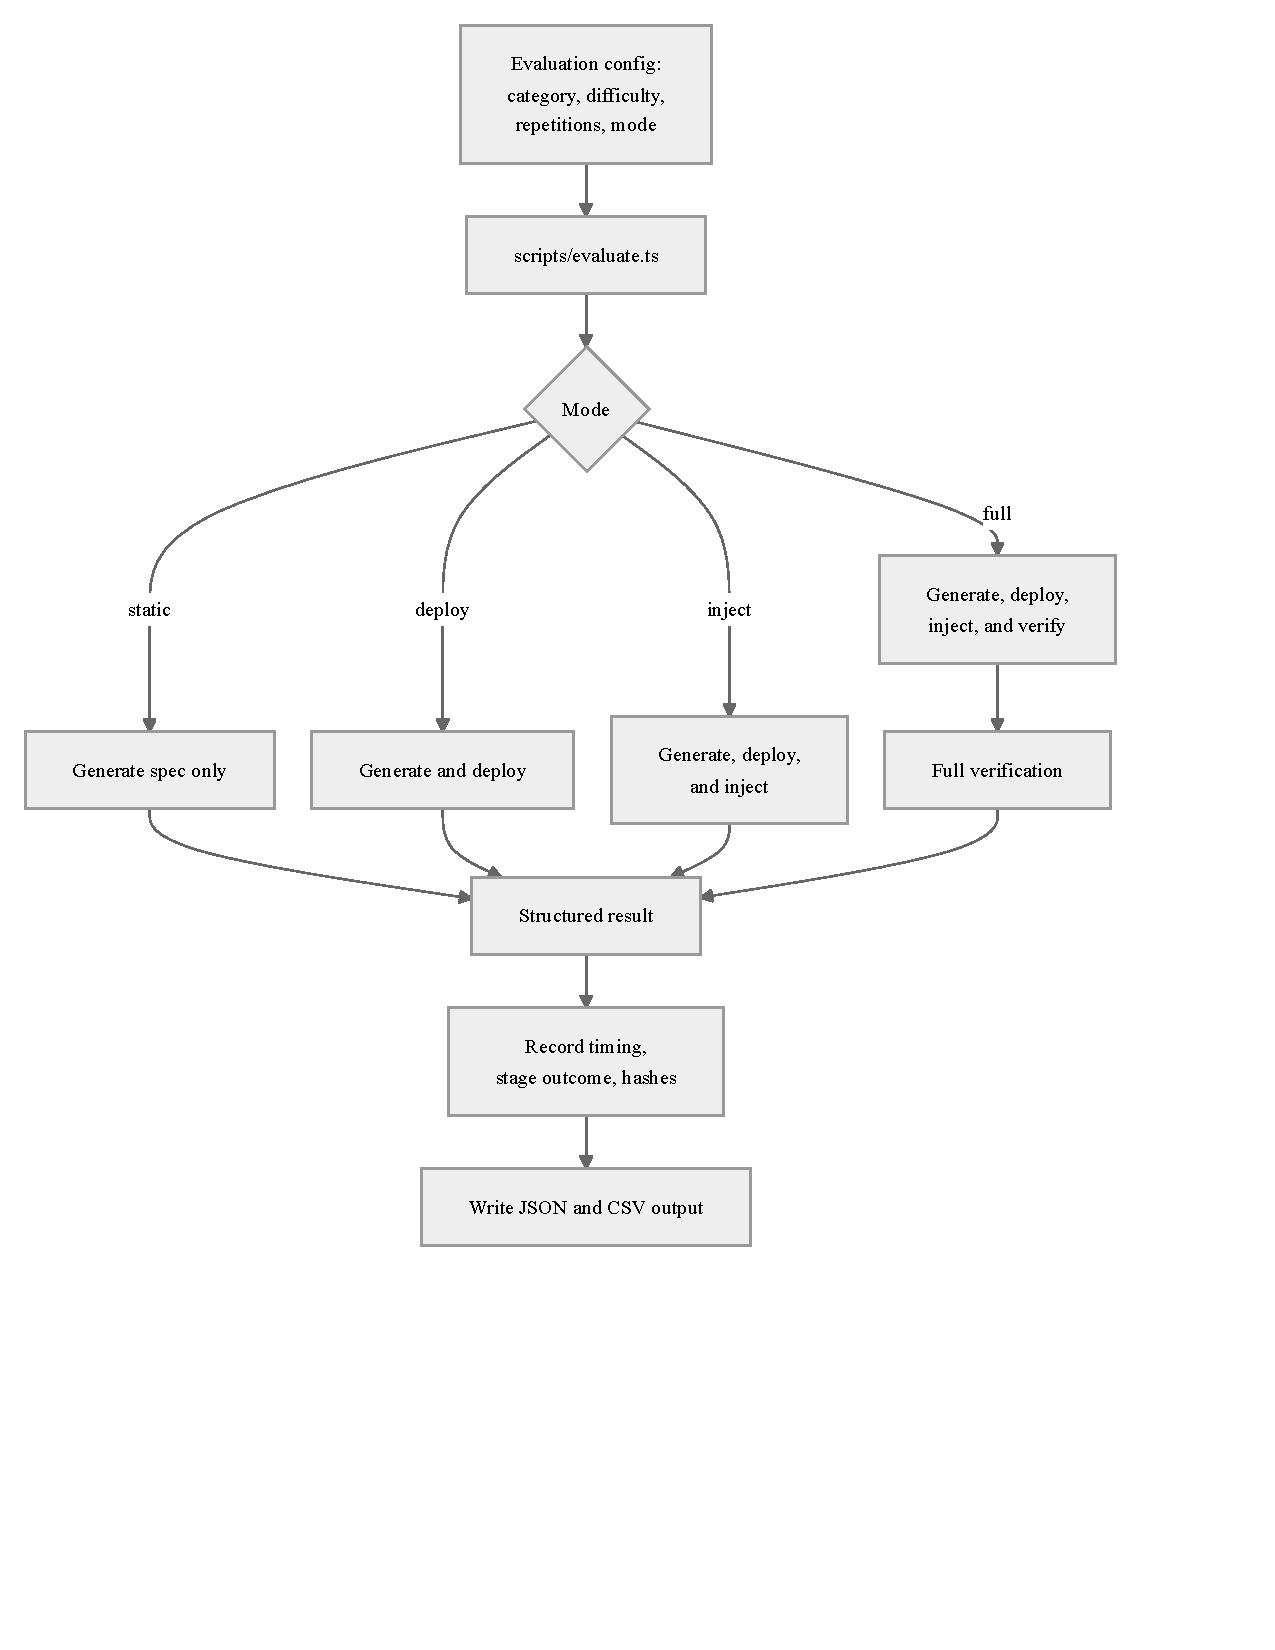
\includegraphics[
		width=\linewidth,
		height=0.82\textheight,
		keepaspectratio
	]{figures/evaluation_harness.pdf}
	\caption{Evaluation Harness}
	\label{fig:evaluation_harness}
\end{figure}

\begin{figure}[htbp]
	\centering
	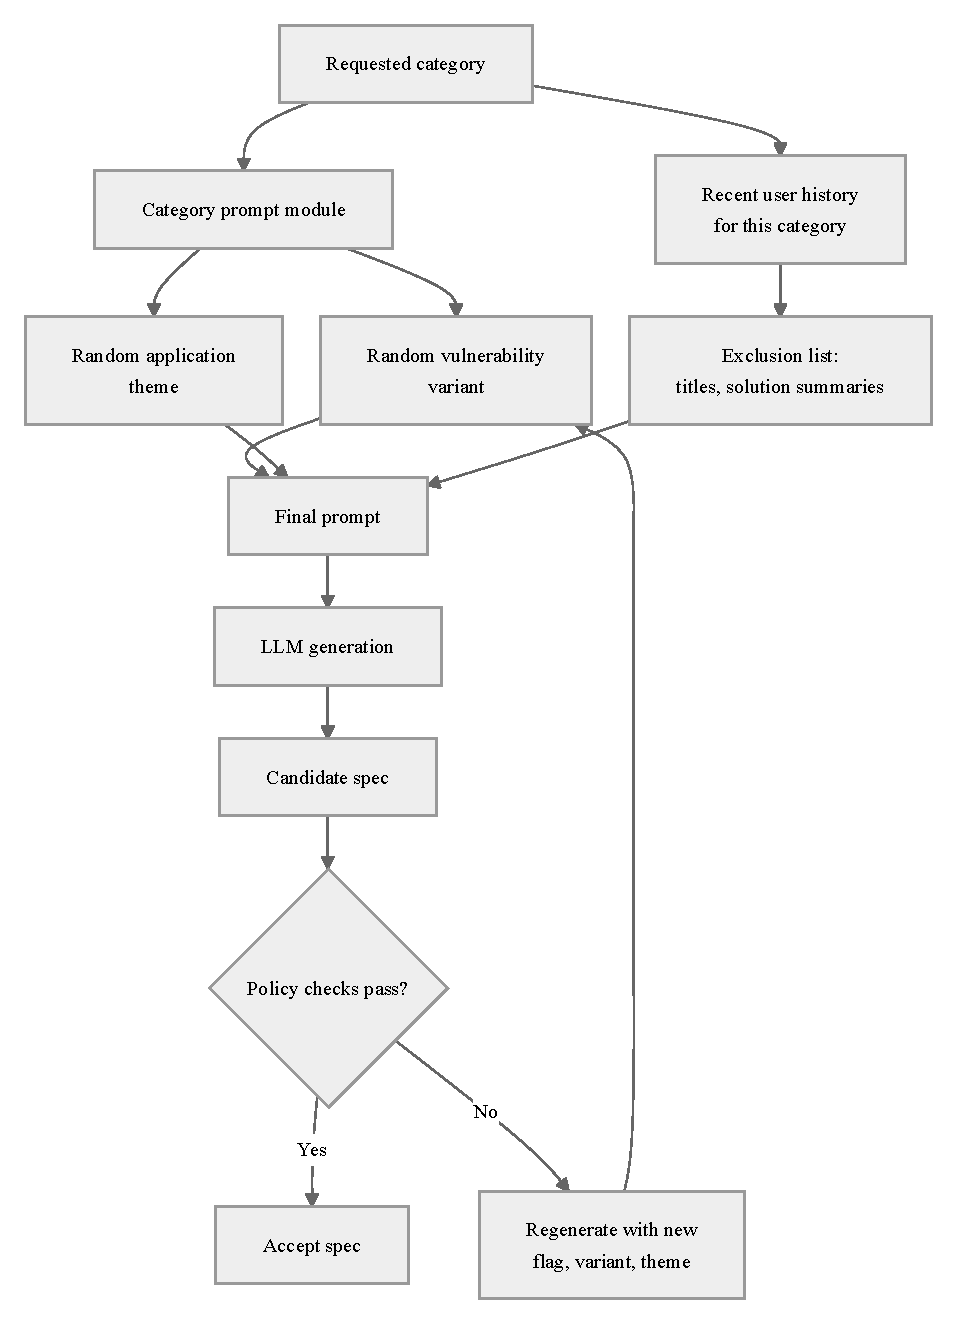
\includegraphics[
		width=\linewidth,
		height=0.82\textheight,
		keepaspectratio
	]{figures/generation_policy.pdf}
	\caption{Prompt Diversity}
	\label{fig:prompt_diversity}
\end{figure}

\section{Further details}\label{app:details}
